\section{数据与评测协议}

\subsection{数据来源}

本文使用两个公开数据集：

\begin{itemize}
  \item \textbf{FaceForensics++ C23}（主库）：1,000 条真人视频与约 6,000 条伪造视频，伪造方法包括 Deepfakes、Face2Face、FaceSwap、NeuralTextures、FaceShifter、DeepFakeDetection。C23 表示 H.264 CRF=23 的中等压缩版本，接近网络传播后的画质。
  \item \textbf{Celeb-DF Test}（跨库）：10,103 张已裁剪人脸图，真 5,036、假 5,067，与 FF++ 的来源、压缩、人脸分布均不同。
\end{itemize}

第三方镜像未提供 DeepFakeDetection 与真人视频一致的源 id，无法做身份配对，因此本文子集实际覆盖 \textbf{5 种伪造方法}。

\subsection{按身份配对抽样}

FF++ 中 \texttt{000.mp4}（真人）与 \texttt{000\_003.mp4}（用 000 生成的假视频）属于同一个人。若按视频随机抽样，同一个人的真假视频可能被分到训练与测试两侧，模型会学习“这张脸是谁”而不是“这张脸是否被改过”，造成身份泄漏、指标虚高。

本文采用\textbf{按身份配对抽样}：先选身份 id，每个身份取 1 条真视频 + 2 条来自不同方法的假视频。初始抽 400 个身份（1,200 条视频），扩展实验再加 300 个身份（900 条视频），最终训练集覆盖 \textbf{580 个身份}。

\subsection{抽帧与人脸对齐}

每条视频按 2 fps 抽帧（FF++ 视频约 10 秒，最多 20 帧），用 OpenCV 的 YuNet 人脸检测器定位最大人脸，外扩 1.4 倍后裁剪为 256$\times$256。最终得到约 2.4 万张（初始）与 4.2 万张（扩展后）人脸帧。裁脸的作用是去除背景干扰，让模型关注面部区域。图~\ref{fig:samples} 给出了真、假样本示例。

\begin{figure}[H]
\centering
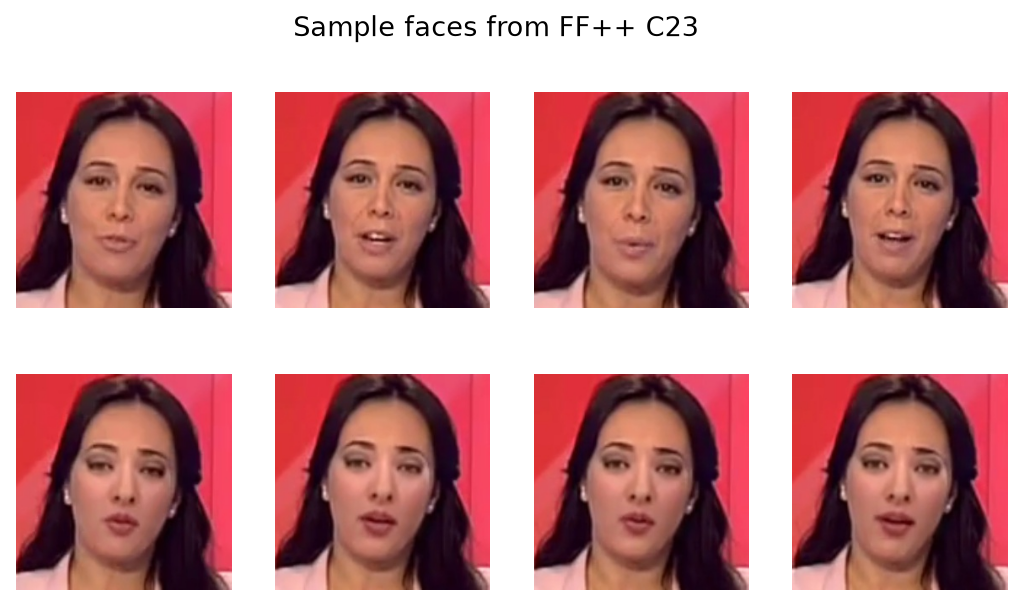
\includegraphics[width=0.92\linewidth]{fig_samples.png}
\caption{FF++ C23 中的人脸样本（上排真、下排假）}
\label{fig:samples}
\end{figure}

\subsection{身份隔离划分}

按源视频 id 分组划分，初始为 280/60/60 个身份，扩展后为 580/60/60。验证集用于选模型与选阈值，测试集只在最终评估时使用。每次划分后检查训练集与测试集的身份交集，必须为 0。

\subsection{退化生成}

为模拟真实传播链，本文实现 6 类退化，见表~\ref{tab:degrade}。训练时以 50\% 概率随机施加 1--2 种退化，评测时按固定参数施加。

\begin{table}[H]
\centering
\caption{评测使用的退化类型}
\label{tab:degrade}
\small
\begin{tabular}{lll}
\toprule
退化 & 参数 & 模拟场景 \\
\midrule
JPEG 重压缩 & 质量 70/50/30 & 社交平台二次压缩 \\
高斯噪声 & $\sigma=5$ & 低质量采集、传输噪声 \\
高斯模糊 & $5\times5$ & 失焦、运动模糊 \\
下采样 & 0.5 倍后再放大 & 低分辨率 \\
随机裁剪 & 裁剪 10\% 后放大 & 构图裁剪、缩放 \\
干净 & 原图 & 对照 \\
\bottomrule
\end{tabular}
\end{table}

\subsection{评测指标与两套口径}

单一阈值下的指标容易掩盖问题，本文同时报告两套口径：

\begin{itemize}
  \item \textbf{部署口径}：用验证集选出的冻结阈值，报告 F1、召回、FPR。阈值在测试集与跨库数据上\textbf{绝不重调}。
  \item \textbf{排序口径}：在测试集 ROC 上取 FPR=1\% 与 FPR=10\% 对应的 TPR（TPR@FPR1\%、TPR@FPR10\%），衡量与阈值无关的排序能力。
\end{itemize}

此外报告 AUC、EER，并对视频做 20 帧平均后的\textbf{视频级}指标。

\subsection{数据规模}

\begin{table}[H]
\centering
\caption{数据规模对比（测试集保持不变，保证可比）}
\label{tab:scale}
\small
\begin{tabular}{lcc}
\toprule
项 & 初始 & 扩展后 \\
\midrule
训练身份 & 280 & 580 \\
验证/测试身份 & 60 / 60 & 60 / 60（不变） \\
训练帧 & 16,800 & 34,719 \\
训练真假比 & 1:2 & 1:2 \\
测试帧 & 3,600（180 条视频） & 3,600（不变） \\
\bottomrule
\end{tabular}
\end{table}

\subsection{处理流程}

图~\ref{fig:pipeline} 给出了从原始视频到评测的完整流程。

\begin{figure}[H]
\centering
\begin{tikzpicture}[
  node distance=6mm,
  box/.style={draw, rounded corners=2pt, align=center, minimum height=9mm, font=\small, fill=gray!6},
  arr/.style={-{Stealth[length=2mm]}, thick}
]
\node[box] (v) {原始视频\\（FF++ C23）};
\node[box, right=of v] (f) {抽帧\\2 fps};
\node[box, right=of f] (c) {YuNet 裁脸\\256$\times$256};
\node[box, right=of c] (s) {按身份\\划分};
\node[box, below=of s] (tr) {训练集\\580 身份};
\node[box, left=of tr] (va) {验证集\\60 身份};
\node[box, left=of va] (te) {测试集\\60 身份};
\node[box, below=of tr] (deg) {随机退化\\50\% 概率};
\node[box, left=of deg] (m) {ResNet18\\训练};
\node[box, left=of m] (e) {多口径评测\\同库/跨库/退化};
\draw[arr] (v) -- (f);
\draw[arr] (f) -- (c);
\draw[arr] (c) -- (s);
\draw[arr] (s) -- (tr);
\draw[arr] (s) -- (va);
\draw[arr] (s) -- (te);
\draw[arr] (tr) -- (deg);
\draw[arr] (deg) -- (m);
\draw[arr] (m) -- (e);
\end{tikzpicture}
\caption{数据处理与评测流程}
\label{fig:pipeline}
\end{figure}
